% !Mode:: "TeX:UTF-8"
%!TEX program  = xelatex

\documentclass[bwprint]{cumcmthesis} 
\usepackage{amssymb}
\usepackage{amsmath}
\usepackage{listings}
\usepackage{graphicx}

\title{第二次校赛建模的题目}

\begin{document}
    \maketitle
    \begin{abstract}
    //摘要//
    \keywords{lweif}
    \end{abstract}
    \section{问题的背景与重述}
        \subsection{引言}
        大巴车交通事故通常将造成比较严重的上伤亡后果。欲避免事故的发生,关键是要有一套行之有效、处罚严厉的管理制度$^{\cite{bib:one}}$。为了使大巴车能够安全运营并有效处理紧急事件,某大巴车出租公司对正在运营的大巴车进行监测。行车记录仪可以每隔一段时间记录从事运营的车辆实际行驶的里程数,若能由此推算出大巴车的任意时刻的速度,并对司机的驾驶水平加以评价与管理,则可达到大大降低运营风险的目的。因此,对该问题的研究具有重要的实际意义。
        \subsection{问题的提出}
        已知$0$-$15$小时内每隔半小时甲、乙、丙三位司机的行驶路程,以及高速公路的限速,建模研究以下问题:
        \begin{enumerate}
            \item 求解三辆大巴车各自运行的速度函数;
            \item 判断三位司机是否有超速行为;
            \item 评价三位司机的驾驶水平。
        \end{enumerate}
    \section{问题分析}
        \subsection{问题一分析}
        问题一要求给出三辆大巴车各自运行的速度函数。注意到题目中所提供的数据为离散取值的若干个数据点,而问题则要求给出一个连续的函数,通常这需要对数据进行拟合等处理来完成。然而,受到信号压缩与重构这一过程的启发,本文采用离散傅里叶变换(DFT)的方法,在已知数据的基础上利用MATLAB软件重构出各车的速度函数。
        首先,将相邻时刻间大巴车行驶的平均速度近似为中间时刻的瞬时速度。其次,利用三次样条插值将数据补充为等时间间隔的点。最后利用快速傅里叶变换(FFT)算法处理数据,在舍去幅度值较低的频率后,重构出所求的速度函数,并检验该函数与原始数据的吻合度。

        \subsection{问题二分析}
        问题二要求判断三位司机是否有超速行为。根据问题一所求出的结果,即可判断函数是否存在某一点使得该时刻的速度大于高速公路的限速。更进一步,还可根据速度函数求出各司机处于超速状态下的总时长。
        \subsection{问题三分析}
        问题三要求评价三位司机的驾驶水平,此题需要建立一个评价模型。首先,选取评价司机的指标。本文选取了司机驾驶的平均速度作为整体速度的衡量;选取每隔半小时行驶里程的样本变异系数衡量数据的分散程度;并选取司机处于超速状态下的时间长度作为司机驾驶的安全程度。在此基础上对司机的驾驶水平进行评价。
        其次,选择评价模型。常用的评价模型有层次分析法、灰色关联度分析以及模糊综合评价法等,考虑到层次分析法在构造判断矩阵时受专家的主观影响较大,导致最终评估结果不符合实际$^{\cite{bib:two}}$,而灰色关联度分析则要求样本数据具有时间序列的特性,故本文采用了模糊综合评价法,分别通过熵权法与层次分析法确定三个指标的客观权重与主观权重,进而确定组合权重。再确定评语集,构造模糊关系矩阵,最终对三个司机的驾驶水平给出评价。
    \section{模型的假设}
        为了...,现做出如下假设:
        \begin{enumerate}
            \item 大巴车在高速公路上行驶,可以不用考虑停车情况;
            \item 大巴车的速度函数为定义在$[0,15]$上的一阶连续可导函数;
            \item 所测得的数据准确无误。
        \end{enumerate}
    \section{主要符号说明}
        \begin{tabular}{cc}
            \hline
            符号	&  意义 \\ \hline
            $F$    & 球受到力的大小 \\ \hline
        \end{tabular}
    \section{模型的原理}
        \subsection{离散傅里叶变换(Discrete Fourier Transform, DFT)}
        在被采样信号和周期信号测量处理中,离散傅里叶变换得到广泛的应用$^{\cite{bib:three}}$。离散傅里叶变换是傅里叶变换的离散形式,即在时域和频域上都呈离散的取值。在形式上,时域和频域上变换两端的序列是有限长的,而实际上这两组序列都被认为是离散的经周期延拓后的信号的主值序列。DFT的公式为:
        \begin{equation*}
            1+1=2
        \end{equation*}
        其中,XXXXXX
        在本文中,采用快速傅里叶变换(Fast Fourier Transform, FFT)算法进行计算。该算法利用了DFT中的奇偶性与虚实性极大地简化了计算,将DFT中$\mathcal{O}(N^2)$的计算量减小至FFT的$\mathcal{O}(NLog2N)$,使得计算机得运算时间大大缩短。

        \subsection{熵权法(Entropy Weight Method, EWM)}
        熵权法是一种根据各项指标观测值所提供的信息量的大小来确定指标权重的方法$^{\cite{bib:four}}$。若某个指标的信息熵越小,表明指标值得变异程度越大,提供的信息量越多,在综合评价中所能起到的作用也越大,其权重也就越大。因此,可利用信息熵这个工具,计算出各个指标的权重,熵权法也由此而来。其计算步骤如下:
        \begin{enumerate}
            \item 数据标准化;(式子)
            \item 求个指标得信息熵;(式子)
            \item 确定各指标的权重。(式子)
        \end{enumerate}
        
        \subsection{层次分析法(Analytic Hierarchy Process, AHP)}
        层次分析法是确定指标主观权重最常用的方法,其主要思想是以评价目标为出发点,对各评价指标进行分解,构造出指标之间的层级关系,再结合判断矩阵计算权重系数$^{\cite{bib:five}}$。其基本步骤如下:
        \begin{enumerate}
            \item 构造判断矩阵;(式子)
            \item 确定各指标权重;(式子)
            \item 一致性检验。(式子)
        \end{enumerate}

        \subsection{模糊综合评价法}
        模糊综合评价是一种基于模糊数学的评价方法,根据模糊数学的隶属度理论把定性评价转化为定量评价,能较好地解决模糊的、难以量化的问题$^{\cite{bib:six}}$。本文按如下步骤求解该模型:
        \begin{enumerate}
            \item 建立评语集并划分评价等级;
            \item 计算指标对各评语的隶属度,进而构造模糊评价矩阵;
            \item 根据先前确定的权重,计算模糊评价向量。
        \end{enumerate}
    \section{模型的求解}
        \subsection{数据的预处理}
        题目要求给出大巴车的速度函数。为将问题简化,首先将题目中的原始数据进行预处理。将相邻半小时内大巴车行驶的平均速度近似为大巴车在中间时刻的平均速度,这样,我们得到$t=0.25, 0.75, 1.25,\dots, 14.75h$共$30$个时刻大巴车的瞬时速度,如下图所示:

        \begin{figure}[ht]
            \centering
            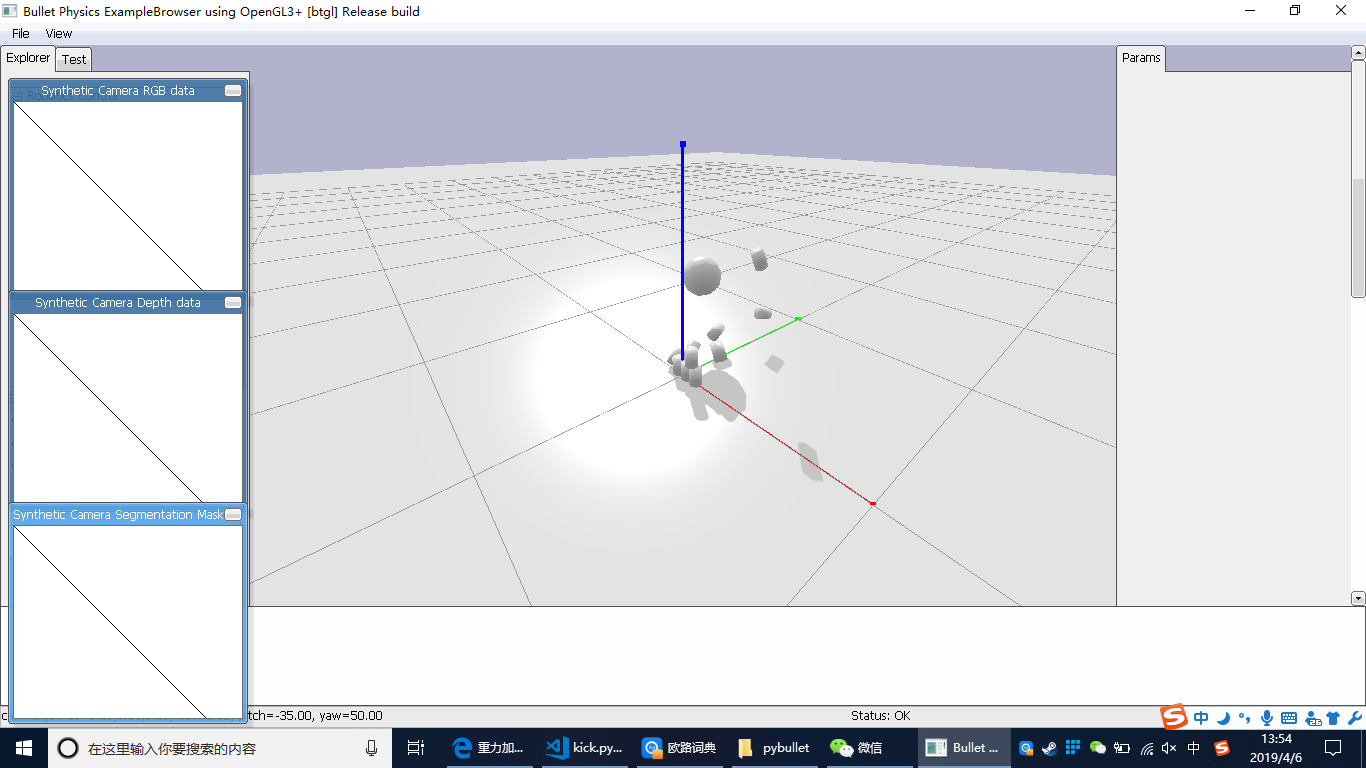
\includegraphics[width=0.8\linewidth]{test.png}
            \caption{label}
        \end{figure}
            
        为方便后续的数据处理,采用三次样条插值的方法,对速度函数$v(t)$进行插值,得到插值后$t=0, 0.5, 1,\dots, 30h$时刻的瞬时速度值。这样我们得到一系列等时间间隔的瞬时速度的数据点,如下图所示:

        \begin{figure}[ht]
            \centering
            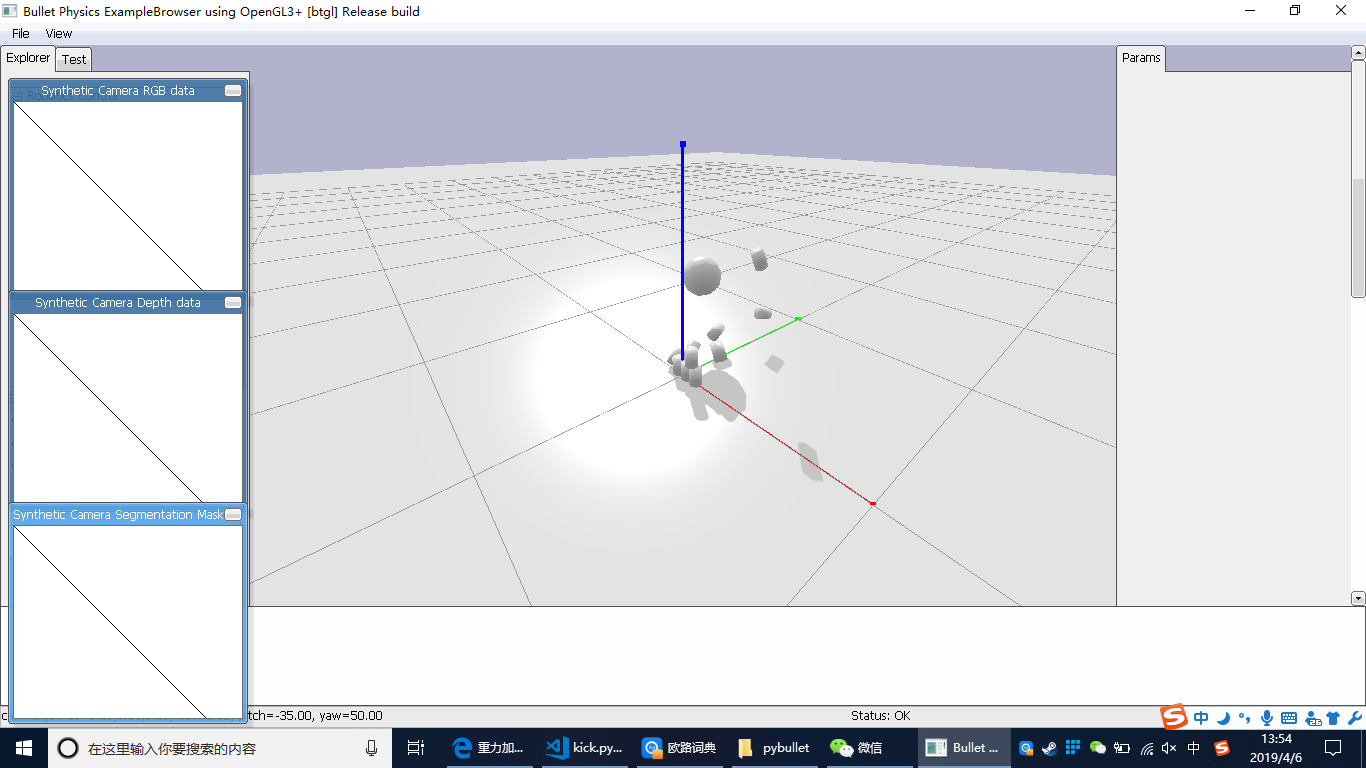
\includegraphics[width=0.8\linewidth]{test.png}
            \caption{label}
        \end{figure}
        
        \subsection{基于FFT的速度求解}
        经过对速度函数$v(t)$的采样,我们即可利用FFT重构出完整的速度函数。下文将$v(t)$假想为定义域为$[0,1]$的信号进行求解,最后只需对时间轴进行拉伸变换即可得到所求的函数。现已将信号以$F_s=60\mathrm{Hz}$的采样频率进行采样,采样点数$N=60$,故FFT所得结果的第$n$个点代表的频率为$F_n=\frac{(n-1)F_s}{N}$。在MATLAB中,利用FFT算法对该序列进行离散傅里叶变换(具体代码见附录),并对得到的$N$个复数$a_n+b_ni$取模,得到各频率值下的幅度特性$A_n$,如下图所示:
        \begin{figure}[ht]
            \centering
            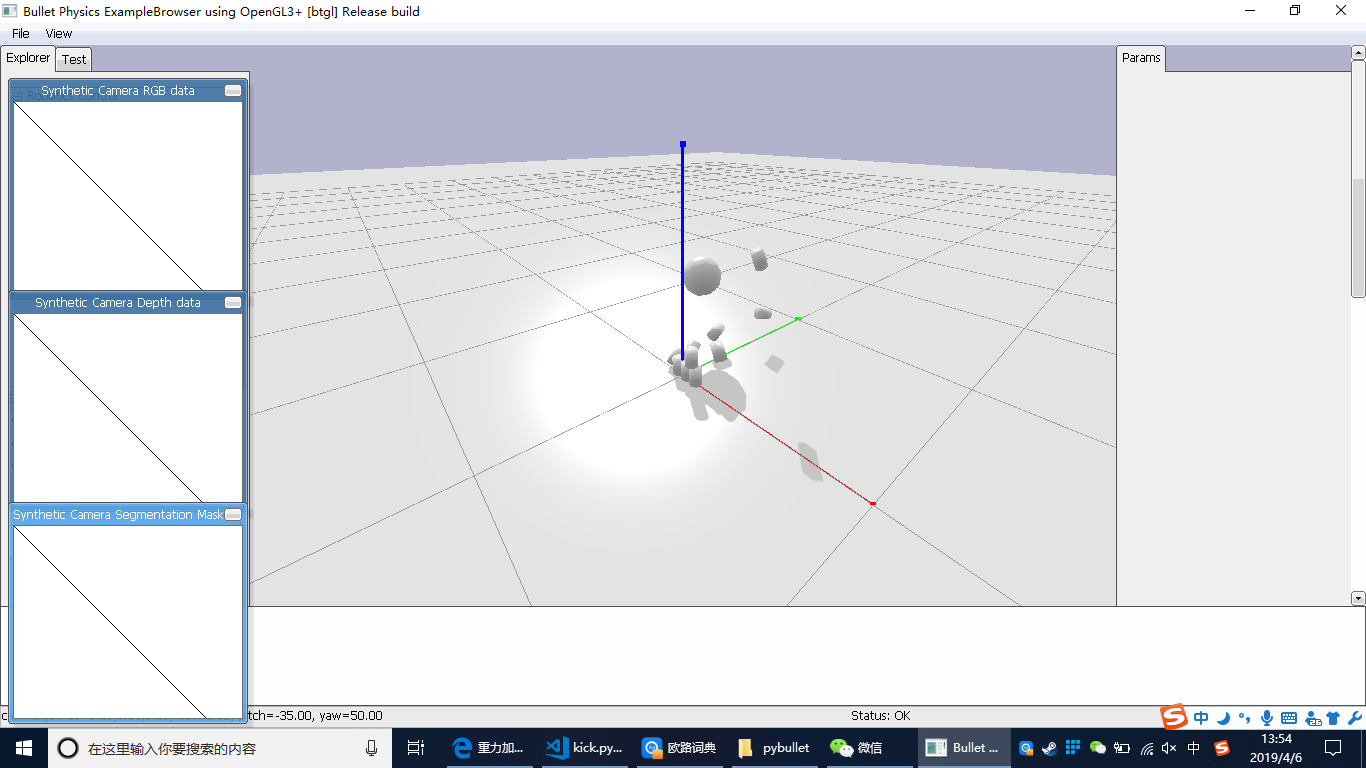
\includegraphics[width=0.8\linewidth]{test.png}
            \caption{label}
        \end{figure}
        通过如上结果,我们进一步得到$n=1$处点的信号直流分量$\frac{A_1}{N}$,以及$2\leq n\leq \frac{N}{2}$时,$n\mathrm{Hz}$信号的幅度$\frac{A_n}{\frac{N}{2}}$,且其相位为$\arctan\frac{b_n}{a_n}$。故我们得到: 
        \begin{equation*}
            v^*(t)=XXX
        \end{equation*}
        最终得到的速度函数可以写成如下形式:
        \begin{equation*}
            v^*(t)=XXX
        \end{equation*}
        其图像大致如下:
        \begin{figure}[ht]
            \centering
            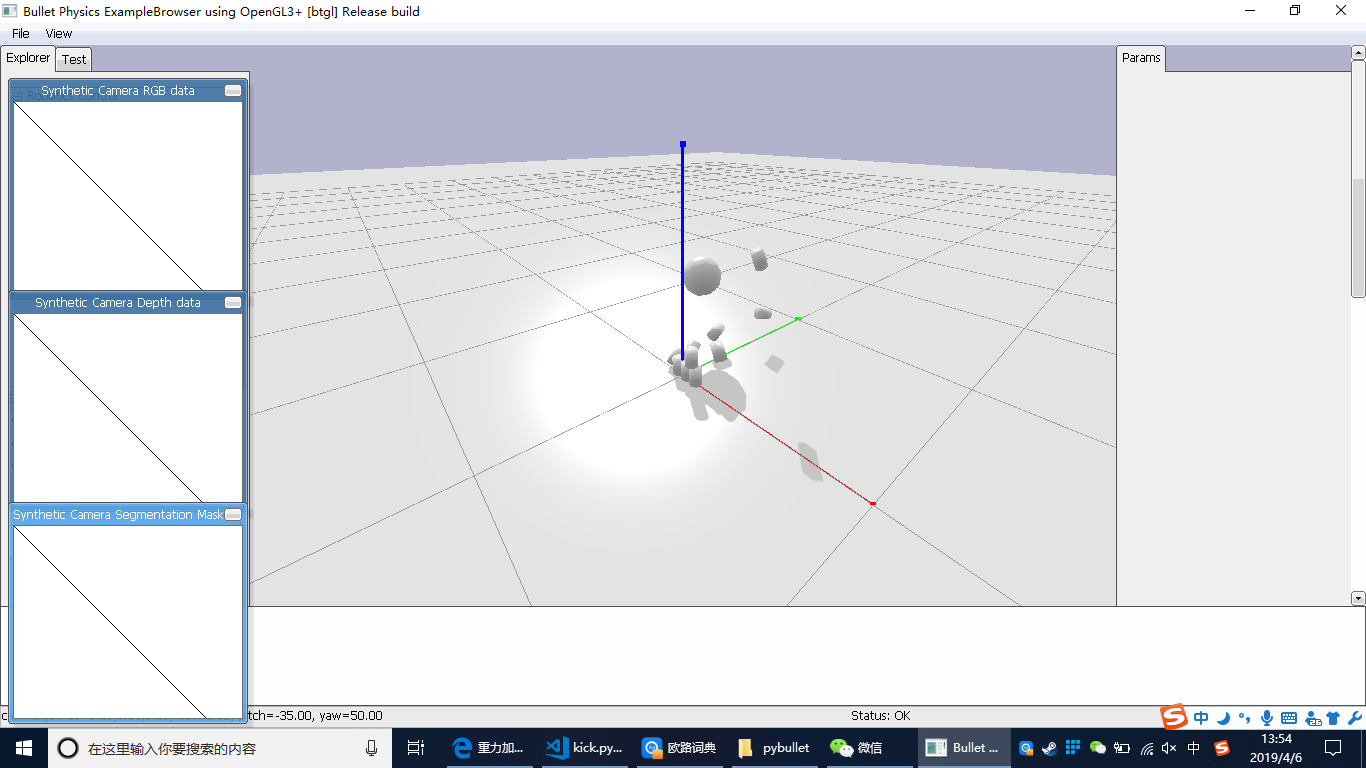
\includegraphics[width=0.8\linewidth]{test.png}
            \caption{label}
        \end{figure}
        

        \subsection{模型的检验}
            现在,对所求出的速度函数与原始数据的吻合度进行检验。分别对相邻半小时下的速度函数进行积分,求出相邻时间里大巴车行驶路程的模拟值,并与实际值加以比较。      \begin{figure}[ht]
                \centering
                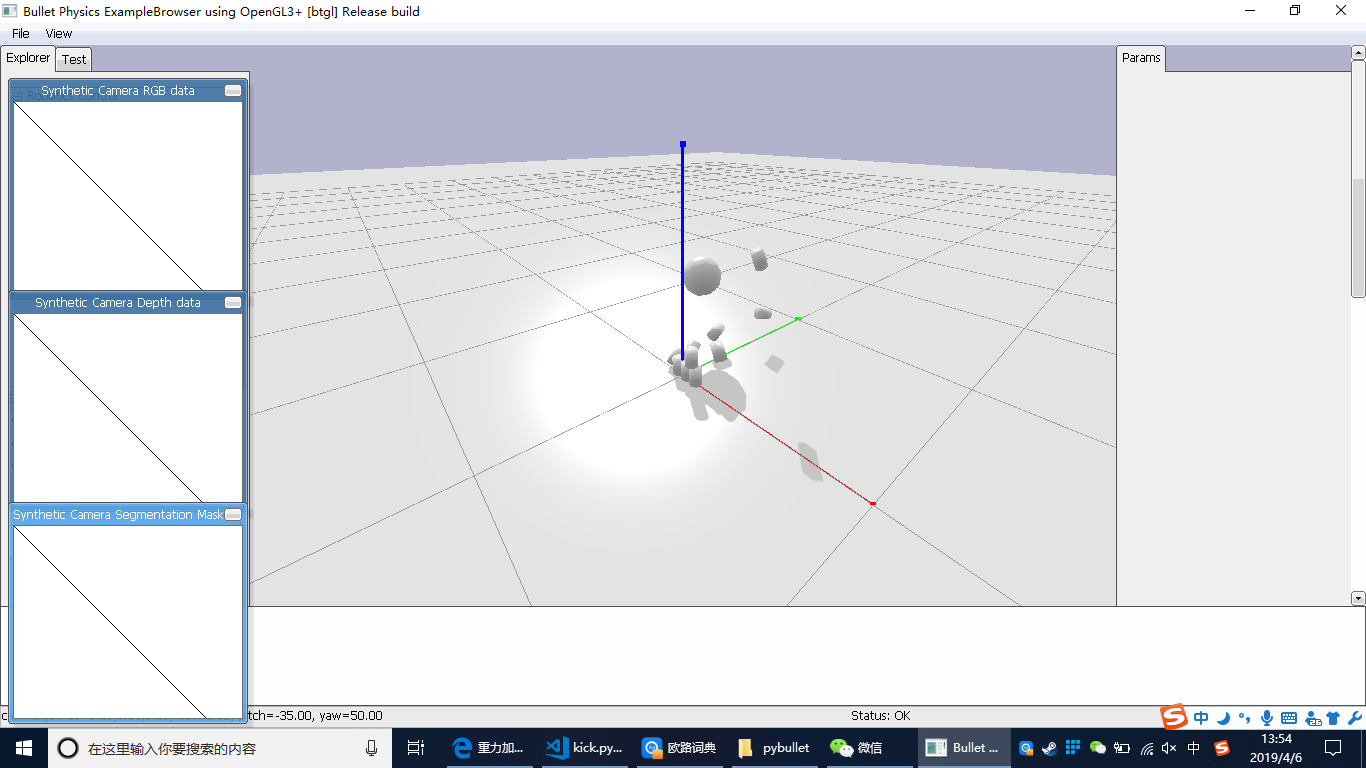
\includegraphics[width=0.8\linewidth]{test.png}
                \caption{label}
            \end{figure}
            经计算,XXXXXXXXXXXXXXXXXXX  //误差分析// 
        
            因此,本文建立的模型是有效可靠的。
        
        \subsection{超速行为的判定}
        将问题一中求得的速度函数与高速公路的限速画入同一张图像中:
        \begin{figure}[ht]
            \centering
            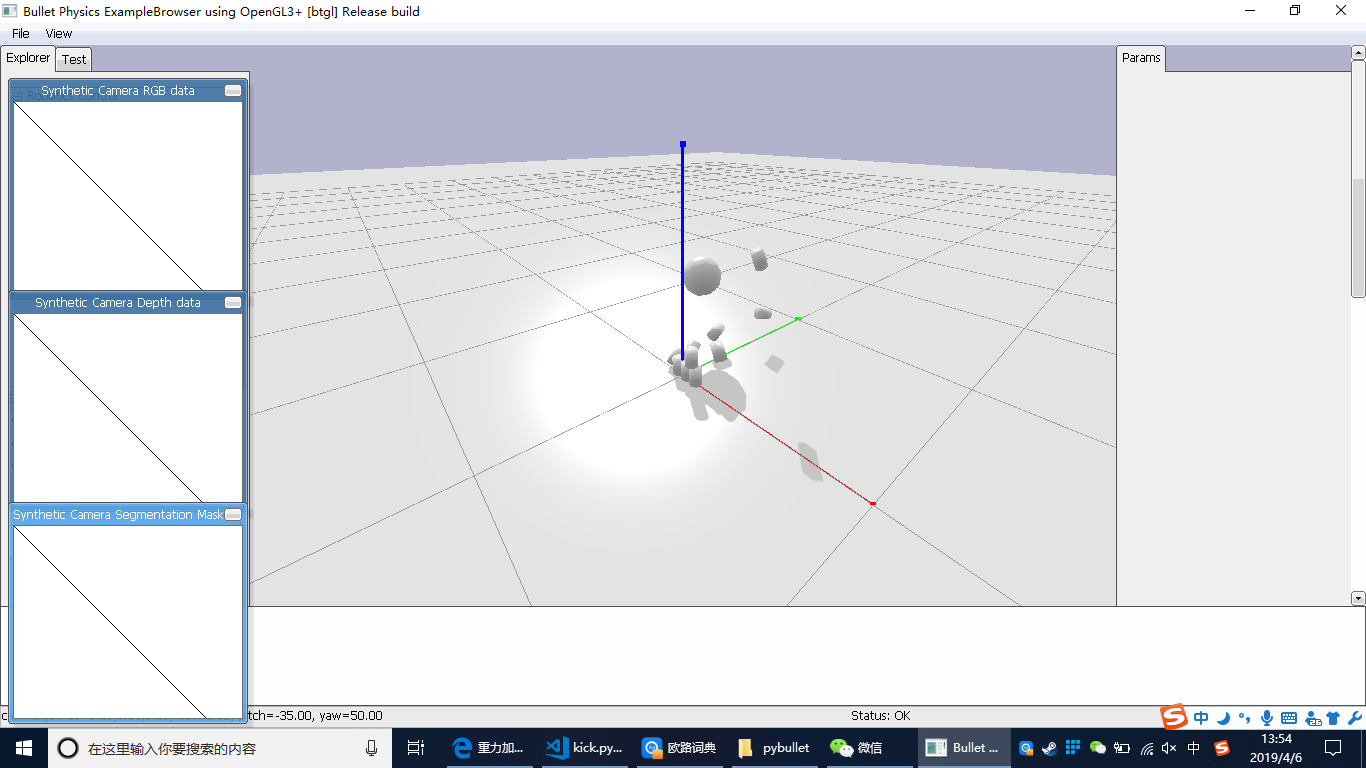
\includegraphics[width=0.8\linewidth]{test.png}
            \caption{label}
        \end{figure}
        可清晰地看出甲、乙、丙三位司机均存在超速的行为。更进一步地,可以求解得出三位司机超速的时间分别为$0.99$小时、$4.455$小时与$2.55$小时。

        \subsection{司机驾驶水平的评价}
        考虑到大巴车出租公司运营中对车辆行驶快速、平稳和安全的实际需求,本文分别选取平均速度、每半小时行驶里程的样本变异系数和超速时间作为衡量三项要求的指标。其中,样本变异系数的计算公式为:
        \begin{equation*}
            1+1=2
        \end{equation*}

        由此,我们得到三位司机驾驶个各项指标如下表:
        
        \begin{tabular}{cc}
            \hline
            符号	&  意义 \\ \hline
            $F$    & 球受到力的大小 \\ \hline
        \end{tabular}

            \subsubsection{基于熵权法的客观权重确定}
            \subsubsection{基于层次分析法的主观权重确定}
            \subsubsection{基于模糊综合评价法的驾驶水平评价}
    \section{模型的评价与改进}
    \subsection{模型的评价}
    //模型的评价//
    \subsection{模型的改进空间}
    //模型的改进空间//
    \begin{thebibliography}{9}
        \bibitem{bib:one} ....
        \bibitem{bib:two} ....
        \bibitem{bib:three} ....
        \bibitem{bib:four} 蔡文军,李晓松.海军舰船装备保障能力评估理论与方法[M]
        \bibitem{bib:five} ....
        \bibitem{bib:six} ....
        
    \end{thebibliography}
    \newpage
    \appendix
        \section{matlab源码}
        \begin{lstlisting}[language=matlab]
            print("Hello world!")
        \end{lstlisting}

\end{document} 